\section{Network device drivers}

\begin{frame}{NIC and MAC}
	\begin{itemize}
		\item Terms \textbf{NIC} and \textbf{MAC} are sometimes used interchangeably
		\item \textbf{N}etwork \textbf{I}nterface \textbf{C}ontroller, usually refers to "Network Cards"
			\begin{itemize}
				\item MAC and PHY integrated in a single component. Usually, the PHY is transparent
			\end{itemize}
		\item On embedded systems, we control each individual component
	\end{itemize}
	\begin{center}
	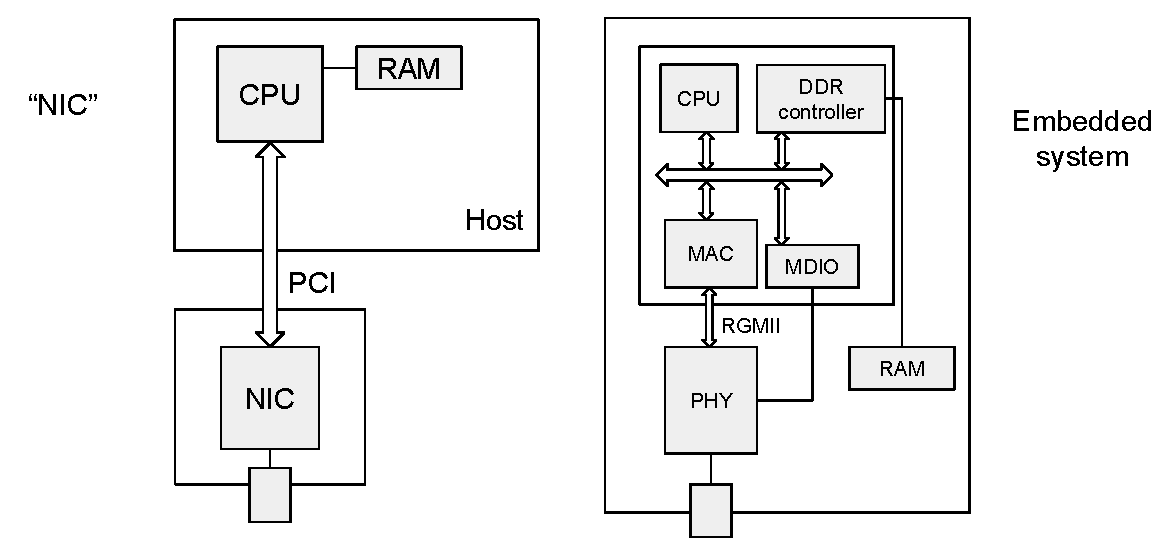
\includegraphics[width=0.8\textwidth]{slides/networking-driver-overview/nic.pdf}
	\end{center}
\end{frame}


\begin{frame}{Low level networking components}
	\begin{itemize}
		\item Multiple drivers are involved to configure a Network Interface
		\item Not all of them are required (depending on the design)
		\item Some MAC drivers also include DMA, Serdes, PCS and even PHY drivers
	\end{itemize}
	\begin{center}
	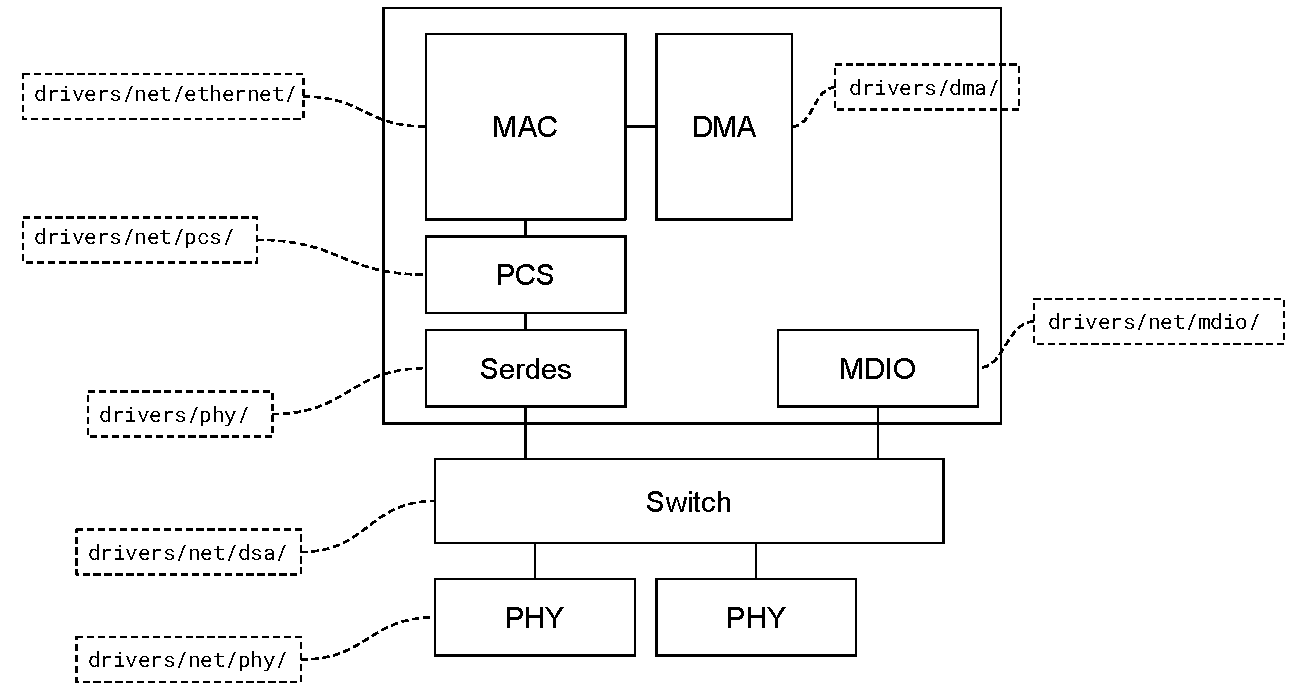
\includegraphics[width=0.8\textwidth]{slides/networking-driver-overview/net_drivers.pdf}
	\end{center}
\end{frame}

\begin{frame}{Low level networking components - MAC}
	\begin{columns}
		\column{0.3\textwidth}
			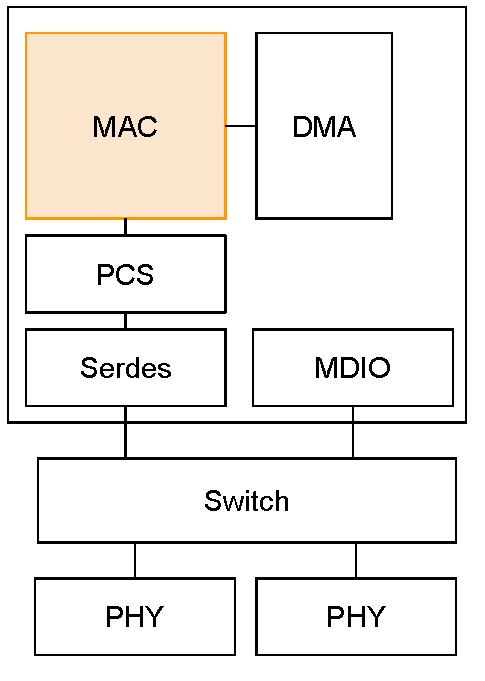
\includegraphics[width=\textwidth]{slides/networking-driver-overview/net_components_mac.pdf}
		\column{0.7\textwidth}
		\begin{itemize}
			\item The main component of a network interface
			\item Represented by \kstruct{net_device}
			\item Drivers are in \kdir{drivers/net/ethernet}
			\item In charge of \textbf{Sending} and \textbf{Receiving} frames
			\item Configures all the \textbf{Hardware offloaded} features
			\item Reports status and statistics
			\item Some devices include a PCS, Serdes, MDIO, PHY, DMA and even a Switch controller in the MAC
				\begin{itemize}
					\item The single MAC driver handles it all
				\end{itemize}
		\end{itemize}
	\end{columns}
\end{frame}

\begin{frame}{Low level networking components - DMA}
	\begin{columns}
		\column{0.3\textwidth}
			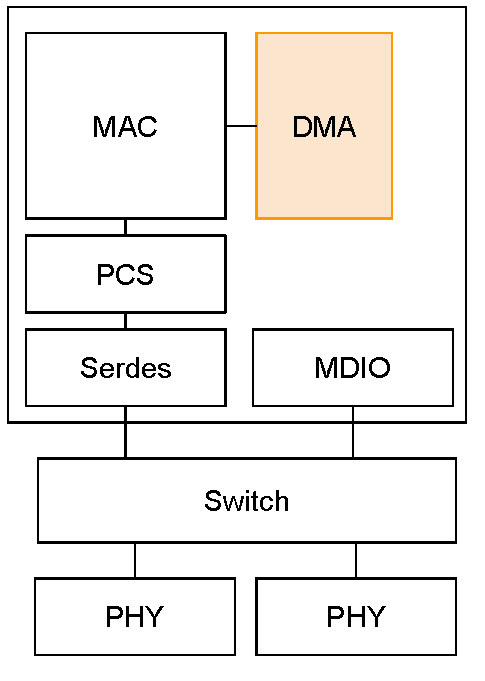
\includegraphics[width=\textwidth]{slides/networking-driver-overview/net_components_dma.pdf}
		\column{0.7\textwidth}
		\begin{itemize}
			\item Some MAC controllers are connected to a shared \textbf{DMA Controller}
			\item The controller handles DMA transfers for multiple devices
			\item The MAC requests \kstruct{dma_chan} for TX and RX
				\begin{itemize}
					\item This is done using the \textbf{dmaengine} API
				\end{itemize}
			\item Drivers are in \kdir{drivers/dma}
			\item It is not unusual to have MAC with an integrated DMA controller
				\begin{itemize}
					\item In that case, we don't use the dmaengine API
				\end{itemize}
		\end{itemize}
	\end{columns}
\end{frame}

\begin{frame}{Low level networking components - PCS}
	\begin{columns}
		\column{0.3\textwidth}
			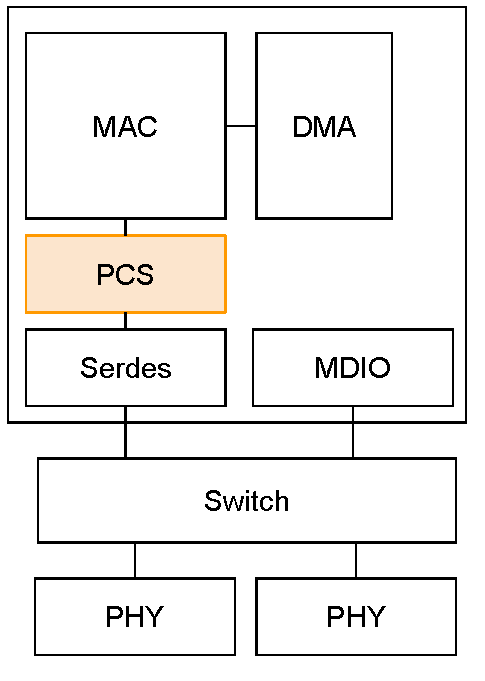
\includegraphics[width=\textwidth]{slides/networking-driver-overview/net_components_pcs.pdf}
		\column{0.7\textwidth}
		\begin{itemize}
			\item \textbf{P}hysical \textbf{C}oding \textbf{S}ublayer
			\item Represented by \kstruct{phylink_pcs}
			\item Drivers in \kdir{drivers/net/pcs}
			\item Component in charge of Data Encoding
				\begin{itemize}
					\item For signal integrity, bits are encoded into symbols
					\item At 100Mbps : 4 bits data, 5 bits symbols (4b/5b)
					\item At 1000Mbps : 8b/10b
					\item At 10Gbps : 64b/66b
				\end{itemize}
			\item Also in charge of in-band signaling
				\begin{itemize}
					\item Link status, speed, duplex, flow-control
				\end{itemize}
			\item Can be transparently handled by the MAC (no driver)
			\item The MAC driver may register its own PCS instance(s)
			\item Some IPs are re-used across vendors, dedicated drivers are then used
		\end{itemize}
	\end{columns}
\end{frame}

\begin{frame}{Low level networking components - Generic PHY}
	\begin{columns}
		\column{0.3\textwidth}
			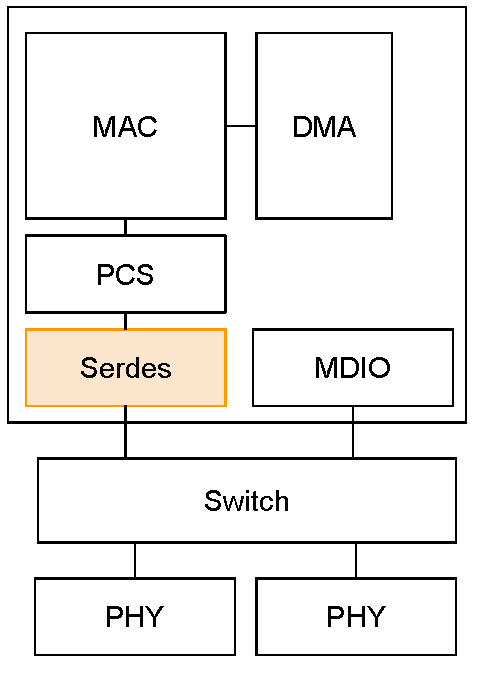
\includegraphics[width=\textwidth]{slides/networking-driver-overview/net_components_serdes.pdf}
		\column{0.7\textwidth}
		\begin{itemize}
			\item Generic PHY, driving the physical link that come out of the MAC
			\item Represented by \kstruct{phy}
			\item Drivers in \kdir{drivers/phy}
				\begin{itemize}
					\item Not to be confused with \kdir{drivers/net/phy}
				\end{itemize}
			\item Usually drives \textbf{SerDes} lanes if the MAC interface is serialized
			\item Also used by other subsystems : USB, PCI, Sata, etc.
			\item Controls the physical link parameters
				\begin{itemize}
					\item Drive strength
					\item Timings
					\item link training, etc.
				\end{itemize}
			\item Sometimes transparently handled by the MAC without a dedicated driver
		\end{itemize}
	\end{columns}
\end{frame}

\begin{frame}{Low level networking components - MDIO}
	\begin{columns}
		\column{0.25\textwidth}
			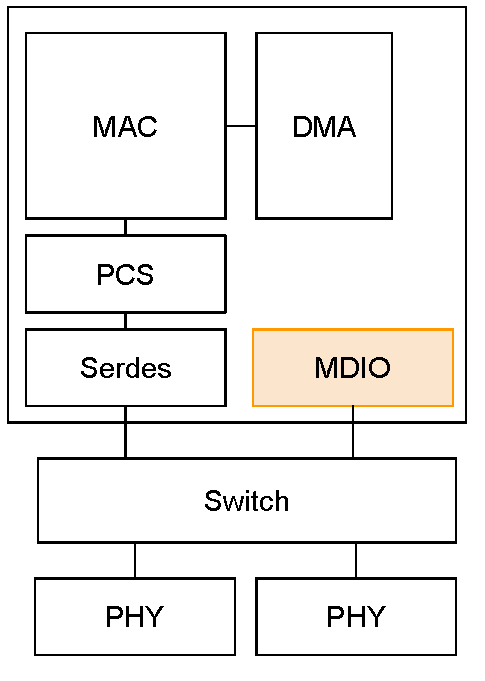
\includegraphics[width=1.1\textwidth]{slides/networking-driver-overview/net_components_mdio.pdf}
		\column{0.75\textwidth}
		\begin{itemize}
			\item \textbf{M}anagement \textbf{D}ata \textbf{I}nput \textbf{O}utput
				\begin{itemize}
					\item a.k.a. \textbf{SMI} : \textbf{S}erial \textbf{M}anagement \textbf{I}nterface
					\item a.k.a. \textbf{MIIM} : \textbf{M}edia \textbf{I}ndependent \textbf{I}nterface \textbf{M}anagement
				\end{itemize}
			\item Bus controller represented by \kstruct{mii_bus}
			\item Peripherals represented by \kstruct{mdio_device}
			\item Drivers in \kdir{drivers/net/mdio}
			\item Management bus for most Ethernet PHYs and DSA Switches
				\begin{itemize}
					\item Only bus for PHYs
					\item Some DSA switches can be controlled by SPI or I²C
				\end{itemize}
			\item Provides ways to access registers, physically similar to I²C
			\item Often controlled by the MAC driver, but can be standalone
		\end{itemize}
	\end{columns}
\end{frame}

\begin{frame}{Low level networking components - Switch}
	\begin{columns}
		\column{0.3\textwidth}
			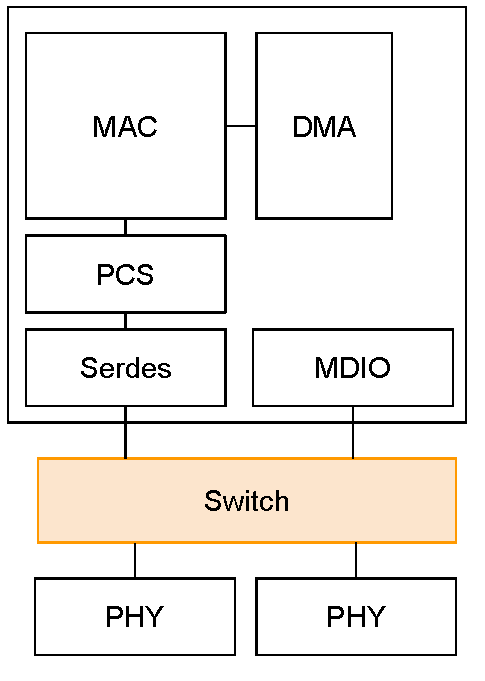
\includegraphics[width=\textwidth]{slides/networking-driver-overview/net_components_switch.pdf}
		\column{0.7\textwidth}
		\begin{itemize}
			\item DSA Switches are standalone chips, with one more ports connected to the SoC's MAC
				\begin{itemize}
					\item \textbf{D}istributed \textbf{S}witch \textbf{A}rchitecture
					\item Relies on \href{https://docs.kernel.org/networking/switchdev.html}{switchdev} for the switching operations
				\end{itemize}
			\item Switches can also be integrated within the SoC
				\begin{itemize}
					\item The MAC driver implements the switchdev operations
				\end{itemize}
			\item DSA switch represented by \kstruct{dsa_switch}
			\item DSA switch port represented by \kstruct{dsa_port}
			\item Switch port represented by \kstruct{net_device} (even for DSA)
			\item Drivers in \kdir{drivers/net/dsa} and \kdir{drivers/net/ethernet}
		\end{itemize}
	\end{columns}
\end{frame}

\begin{frame}{Low level networking components - Ethernet PHY}
	\begin{columns}
		\column{0.3\textwidth}
			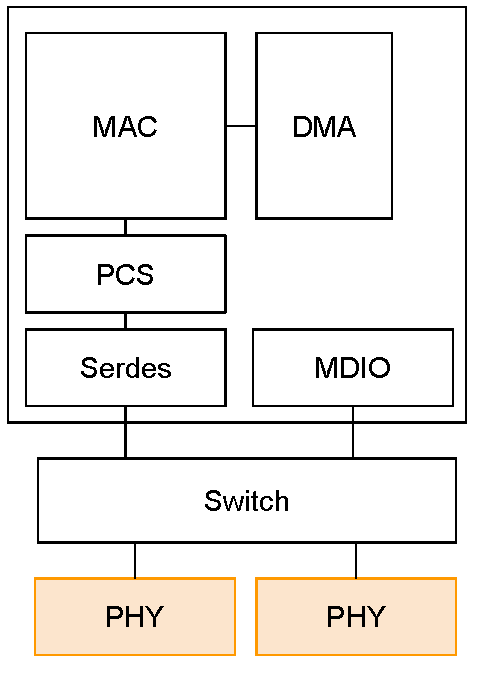
\includegraphics[width=\textwidth]{slides/networking-driver-overview/net_components_phy.pdf}
		\column{0.7\textwidth}
		\begin{itemize}
			\item In charge of 802.3 Layer 1 (PHY) operations
			\item Represented by \kstruct{phy_device}
			\item Drivers in \kdir{drivers/net/phy}
			\item Specific to MDIO PHYs, as per the 802.3 specification
			\item In charge of link management :
				\begin{itemize}
					\item Auto-negociation of Speed and Duplex
					\item Link detection
				\end{itemize}
			\item A generic driver exists using only standard registers
			\item The PHY management framework is called \textbf{phylib}
		\end{itemize}
	\end{columns}
\end{frame}
% NIC components (MAC, PHY, DMA, PCS, SFP, Switch)
